\section{\textsc{Salatsauce mit Sahne}}

\subsection*{Zutaten für 300ml:}

\begin{tabular}{p{7.5cm} p{7.5cm}}
	& \\
	250ml Sahne & Salz, Pfeffer \& edelsüßer Paprika \\
	50ml Zitronensaft & 
\end{tabular}

\subsection*{Serviervorschlag:}

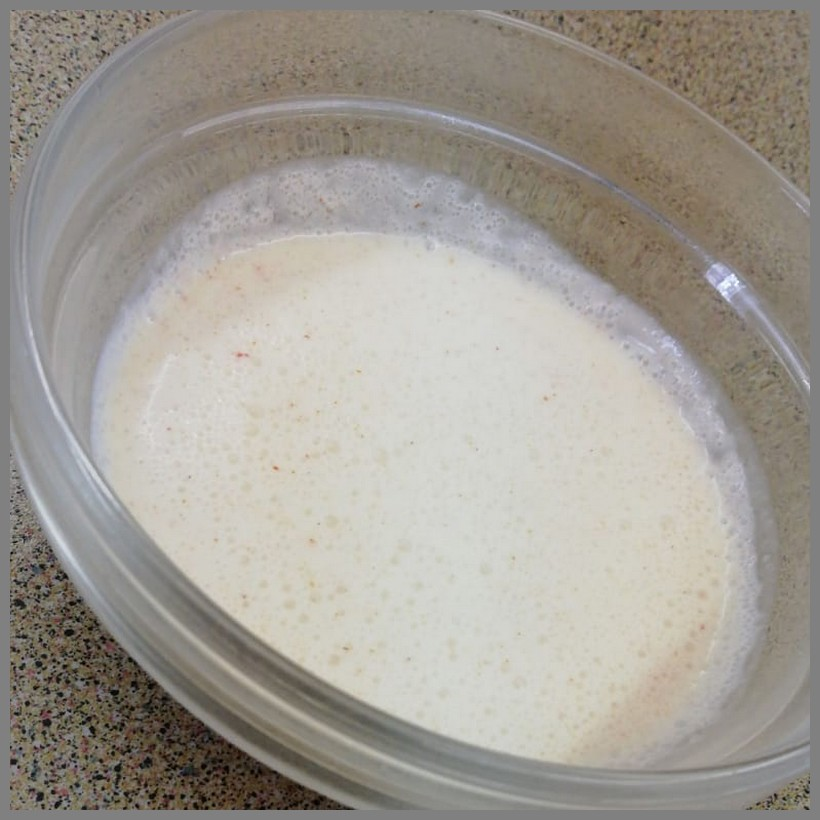
\includegraphics[width=\textwidth]{img/d_sahne.jpeg} \cite{dsahne}

\subsection*{So geht's:}

\begin{tabular}{p{15cm}}
	\\
	Sahne und Saft verrühren und anschliessend mit Gewürzen abschmecken.\\
	\\
	Geeignet zu Blattsalat, Salat mit Obst und Gemüsesalat.
\end{tabular}
